
\section{Implementación de casos de estudio con servicios en la nube existente}
\label{\detokenize{chapter_two/study_cases_implementation:implementacion-de-casos-de-estudio-con-servicios-en-la-nube-existente}}\label{\detokenize{chapter_two/study_cases_implementation::doc}}


\subsection{Reconocimiento de rostros utilizando la API de Kairos}

En la arquitectura utilizamos los servicios de detección de rostros y reconocimiento
de sujetos de la API de Kairos.
Dentro de la aplicación móvil, la API REST de CloudNAO es el intermediario
que se comunica con la API de Kairos, esto es por facilidad y por no
tener que manejar muchas API y SDK por cada servicio que se desee usar.
A pesar de que en el sistema sólo se utiliza el servicio
dentro de la aplicación móvil, es posible ejecutar directamente la clase
\texttt{Kairos} del módulo \texttt{app.tpa\_client\_libraries.kairos\_client}
en el robot (esta clase es parte del la API REST de CloudNAO), para enviar la petición y procesar la respuesta desde éste.
Por ahora sólo se muestra el uso de este servicio en la aplicación móvil.

Cuando el usuario selecciona en el menú de navegación de la aplicación
la tarea de \textbf{Reconocimiento de personas} se muestra una pantalla 
con tres botones, uno para obtener una fotografía del robot, otro para
detectar rostros de nuevas personas, y el tercero para reconocer sujetos
ya almacenados. Si el usuario desea añadir a una nueva persona, se abre un
formulario emergente con un campo para agregar el nombre de la persona y
si no hay errores y la detección se realizó correctamente,
la cara de la persona queda almacenada y se pueden realizar futuros reconocimientos.

Si se desea realizar el reconocimiento de personas cuyo rostro
fue previamente guardado, se presiona el botón con la etiqueta
\textit{Reconoce personas} y si todo sale bien,
se muestra una lista de las personas en la fotografía.
Al dar clic sobre el nombre de la persona en la lista, el robot ejecuta
un movimiento de saludo diciendo una frase simple con el nombre de la persona.

\begin{figure}[htbp]
\centering
\caption{El flujo de el reconocimiento de personas. 1) El usuario presiona el botón para capturar una imagen desde el robot. 2) El robot envía la imagen a la 
aplicación. 3) El usuario presiona el botón Reconoce personas y envía la imagen a la API REST de CloudNAO. 4) La API de CloudNAO solicita el recurso \texttt{recognize} de Kairos. 5) Kairos envía un JSON como respuesta. 6) La API 
de CloudNAO envía un JSON a la aplicación móvil. 7) La aplicación envía ejecuta el remotamente el módulo de NAOqi para realizar el discurso animado.}
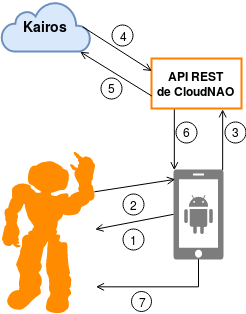
\includegraphics[scale=0.6]{study_case_kairos}
\end{figure}

\subsection{Reconocimiento óptico de caracteres y traducción de texto con Google Cloud Vision y Google Cloud Translation}

El reconocimiento óptico de caracteres (OCR por sus siglas en inglés) permite detectar y extraer texto de imágenes para luego
almacenarlo en un formato que una máquina pueda "entender".
La API de Vision de Google Cloud ofrece el servicio de OCR
que además incluye la detección del idioma en que se encuentra escrito.
Google Cloud cuenta también con una API para traducción de 
texto.
En la API REST de CloudNAO se combinan estos dos servicios
para añadir al robot NAO la funcionalidad de extracción y traducción de texto en imágenes. 

Esta característica dentro de CloudNAO sólo
se usa en la aplicación móvil, sin embargo, al igual que
la el reconocimiento de rostros, se puede utilizar directamente
sobre el robot. El usuario simplemente adquiere una fotografía
capturada por la cámara del robot y se hace la petición
a la API REST de CloudNAO que utiliza los servicios
de Google Cloud Vision y Translation para obtener el texto
y hacer la traducción, respectivamente.
Si existe texto en la imagen y fue correctamente procesado por
la API de Vision, éste se traduce, el resultado se muestra
en la aplicación y el robot repite oralmente
el texto traducido.

\subsection{Reconocimiento de voz con la API de Wit.ai}

Una aplicación interesante de tecnologías que realizan el 
procesamiento de lenguaje natural es la creación de bots conversacionales
o asistentes por voz. Wit.ai provee una API para construir aplicaciones
con las que los usuarios se puedan comunicar a través de voz o texto.
El robot NAO es una plataforma con las características 
para interactuar de manera amigable, que a pesar de contar con un
módulo de reconocimiento de voz (\texttt{ALSpeechRecognition}), éste es muy 
básico y limitado.

Las aplicaciones desarrollados con Wit.ai aprenden conforme reciban más 
información, se vuelven más inteligentes con cada interacción de los usuarios.
En cambio, una aplicación usando sólo el módulo de \texttt{ALSpeechRecognition} es estática.

Por todas estas razones se creó una aplicación sencilla
para interactuar con el robot usando el servicio \texttt{speech} de
Wit.ai.
Dentro de la API REST de CloudNAO existe un módulo para hacer las peticiones
a la API de Wit.ai; éste también puede usarse directamente sobre
el robot, evitando un intermediario.
Se solicita el recurso \texttt{speech} de la API de Wit.ai 
enviando
un archivo de audio generado por el robot. La API
envía como respuesta un JSON con la transcripción del audio 
en texto, las entidades e intenciones encontradas.
El robot es quien se encarga de manejar el flujo de
acciones dependiendo de las entidades.

Las entidades de una aplicación se definen en la plataforma
web de Wit.ai. Ésta cuenta con una herramienta para
crear entidades a partir de oraciones que el usuario
posiblemente enviará en un mensaje. Por ejemplo,
cuando el usuario inicie una conversación posiblemente
se con un "Hola", por lo que podemos definir una
entidad \texttt{saludo} con el valor \texttt{hola}.
Se pueden añadir más sentencias que el usuario
pueda decir cuando quiera saludar como "Buenas tardes",
"Buena día" y la entidad seguirá siendo saludo.
A partir de esto podemos definir acciones muy simples
para el robot guiadas por las entidades. En la
siguiente lista se describen las entidades que se
definieron para esta aplicación, qué acción realiza el robot
y un ejemplo de lo que puede decir el usuario para ejecutarla:


\begin{itemize}
\item  \texttt{walk}: El robot camina una pequeña distancia. "Vamos, camina."
\item \texttt{restPosition}: El robot cambia a una posición de descanso (crouch). "Descansa robot".
\item \texttt{greeting}: El robot realiza un gesto y saluda al usuario."Hola robot".
\item \texttt{photography}: El robot toma una fotografía y la almacena en su disco. "Toma una foto de lo que ves".
\item \texttt{sayGoodbye}: El robot se despide del usuario y termina la aplicación. "Adiós robot".
\item \texttt{animation}: El robot ejecuta una animación aleatoria.
"Robot, dame un movimiento sorpresa".
\item \texttt{textDetection}: Utilizando la API de Vision de Google Cloud
el robot extrae texto de una imagen y lo expresa oralmente. "Lee que dice
aquí".
\end{itemize}

La aplicación se puede volver tan compleja como se desee,
el añadir más entidades hace más interesante intectuar con el
robot. Podemos agregar otros servicios para
que cada vez se parezca más a un asistente por voz,
como los calendarios y contactos de Google, la búsqueda de lugares y
zonas de interés con servicios como Foursquare o los Mapas de Google,
uso de la la gráfica de conocimiento de Google o de Wolfram Alpha, 
servicios de noticias, etc.

\begin{figure}[htbp]
\centering
\caption{El funcionamiento de la interacción con el robot a través de un discurso
oral. 1) El usuario envía un mensaje que el robot graba en un archivo de audio
con unos cuantos segundo de duración. 2) El robot procesa envía el archivo de audio
a la API de Wit.ai. 3) Wit.ai envía un JSON con las entidades encontradas. El robot realiza una acción dependiendo de las entidades.}
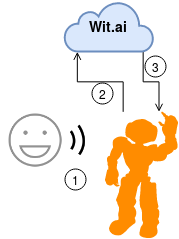
\includegraphics{study_case_wit}
\end{figure}

